%% wp6 逆布局：右逆、左逆及应用（论文 Inverse 小节）
\wpsh{逆（Inverse）}
\label{sec:inverse}

布局可以是单射（injective）、满射（surjective）或双射（bijective）的，并且存在右逆（right-inverse）、左逆（left-inverse）、全逆（full-inverse）与拟逆（quasi-inverse）。当把布局解释为从坐标到偏移的函数时，逆布局便可解释为从偏移到坐标的函数。布局的逆很有用：确定某些偏移在布局中的位置、提取由特定偏移构成的组，或确定两个布局各自的公共子布局。

本节定义布局的广义左逆与右逆，并给出使用它们的应用示例。

\wpssh{右逆（Right-Inverse）}

布局 $\v{L} : \Z_{\abs{\v{L}}} \to \D$ 的{\em 右（伪）逆}是一个单射布局 $\v{L}^{\ddagger} : \D_{\v{L}^{\ddagger}} \to \Z_{\abs{\v{L}}}$，满足
\begin{align}
\forall k \in \D_{\v{L}^{\ddagger}}, \ \ \v{L}^\ddagger(\v{L}(\v{L}^\ddagger(k))) &= \v{L}^\ddagger(k)
\label{eqn:right-inverse}
\end{align}
当 $\v{L}$ 具有一般的整数半模（integer-semimodule）陪域（codomain）$\D$ 时，上述一般性定义可用来刻画 $\v{L}^{\ddagger}$ 的性质。在常见情形 $\D = \Z$ 下，可以恢复出右逆的经典定义，
\begin{align*}
\forall k \in \Z_{\abs{\v{L}^{\ddagger}}}, \ \ \v{L}(\v{L}^{\ddagger}(k)) = k,
\end{align*}
而对于更一般的陪域，例如 $\D = \Z^{(\ast,\ast)}$，由式~\eqref{eqn:right-inverse} 可以推出 $\D \lesssim \v{L}^\ddagger$：右逆的定义域（domain）对 $\v{L}$ 陪域的轮廓做了粗化，使其能够接受来自 $\v{L}$ 的偏移。

若布局 $\v{L}$ 存在右逆布局 $\v{L}^\ddagger$，则 $\abs{\v{L}^\ddagger} \leq \abs{\v{L}}$。实践中，提到某布局的右逆时，我们通常指尺寸最大的那个右逆。例如，图~\ref{fig:layouts} 与图~\ref{fig:layouts2} 中布局的最大尺寸右逆如表~\ref{tab:rinv} 所示。

\begin{table}[ht]
\begin{center}
\begin{tabular}{|>{$}c<{$}|>{$}c<{$}|c|}
\v{L} & \v{L}^\ddagger & \textbf{备注} \\ \hline \hline
(4,8):(1,4) & 32:1 & \\ \hline
(4,8):(8,1) & (8,4):(4,1) \\ \hline
(3,7,5):(5,15,1) & (5,21):(21,1) & 非 2 的幂的形状/步幅也没有问题。 \\ \hline
(4,8):(1,5) & 4:1 & 对非连续的像，结果更小。 \\ \hline
(4,(4,2)):(4,(1,16)) & (4,4,2):(4,1,16) & 结果定义域与陪域 $\Z$ 同余。 \\ \hline
((2,2),(4,2)):((1,8),(2,16)) & (2,4,2,2):(1,4,2,16) \\ \hline
((2,2),(2,4)):((0,1),(0,2)) & (2,4):(2,8) & 步幅为 0 的模没有贡献。 \\ \hline
((2,2),(2,4)):((0,2),(0,4)) & 1:0 & 平凡右逆。 \\ \hline
(4,8):(e_0,e_1) & (4,8):(1,4) & 结果定义域与陪域 $\Z^{(\ast,\ast)}$ 同余。 \\ \hline
(4,(4,2)):(e_1,(e_0,6e_1)) & (4,4):(4,1) & 结果更小且定义域相容。 \\ \hline
(4,(4,3)):(f_1,(f_5,f_{16})) & (4,4,3):(f_1,f_5,f_{16}) & 对整数模步幅也可定义。 \\ \hline
\end{tabular}
\end{center}
\caption{布局右逆的示例。}
\label{tab:rinv}
\end{table}

当布局 $\v{L}$ 是 $\Z_{\abs{\v{L}}}$ 上的双射时，右逆同时也是布局 $\v{L}$ 的{\em 逆} $\v{L}^{-1}$，满足
\begin{align*}
\forall k \in \Z_{\abs{\v{L}}}, \ \ \v{L}(\v{L}^{-1}(k)) = k = \v{L}^{-1}(\v{L}(k))
\end{align*}
若布局 $\v{L}$ 存在全逆 $\v{L}^{-1}$，则称该布局是{\em 紧凑}（compact）的。

\wpssh{应用：向量化（Vectorization）示例}

\begin{figure}[ht]
	\centering
	\begin{subfigure}[t]{0.35\textwidth}
		\centering
		\begin{tikzpicture}[thick,scale=1.10, every node/.style={scale=1.10}]
			\begin{scope}[xshift=-1.5cm]
			\matrix[matrix of nodes,nodes={draw,inner sep=0pt,text width=.5cm,align=center,minimum height=.5cm}]
			at (0,0) {
				0 & 4 & 8  & 12 \\
				1 & 5 & 9  & 13 \\
				2 & 6 & 10 & 14 \\
				3 & 7 & 11 & 15 \\};
			\fill [gray,fill opacity=0.4] (-1.05,0) rectangle (-0.50,1.05);
			\draw (0,-1) node[anchor=north,align=center] {\footnotesize $(4,4):(1,4)$ \\ \footnotesize 源};
			\end{scope}
			\begin{scope}[xshift=+1.5cm]
			\matrix[matrix of nodes,nodes={draw,inner sep=0pt,text width=.5cm,align=center,minimum height=.5cm}]
			at (0,0) {
				0 & 2 & 4  & 6 \\
				1 & 3 & 5  & 7 \\
				8 & 10 & 12 & 14 \\
				9 & 11 & 13 & 15 \\};
			\fill [gray,fill opacity=0.4] (-1.05,0) rectangle (-0.50,1.05);
			\draw (0,-1) node[anchor=north,align=center] {\footnotesize $((2,2),4):((1,8),2)$ \\ \footnotesize 目标};
		    \end{scope}
		\end{tikzpicture}
		\caption{2 元素公共子向量。} \label{fig:autovec1}
	\end{subfigure}
    \quad\quad\quad\quad\quad\quad
	\begin{subfigure}[t]{0.5\textwidth}
	\centering
	\begin{tikzpicture}[thick,scale=1.10, every node/.style={scale=1.10}]
		\begin{scope}[xshift=-2cm]
		\matrix[matrix of nodes,nodes={draw,inner sep=0pt,text width=.5cm,align=center,minimum height=.5cm}]
		at (0,0) {
			0  & 4  & 1  & 5  \\
			8  & 12 & 9  & 13 \\
			2  & 6  & 3  & 7  \\
			10 & 14 & 11 & 15 \\};
		\fill [gray,fill opacity=0.4] (-1.05,+0.50) rectangle (-0.50,1.05);
		\fill [gray,fill opacity=0.4] (-1.05,-0.50) rectangle (-0.50,0.00);
		\fill [gray,fill opacity=0.4] (    0,+0.50) rectangle (+0.50,1.05);
		\fill [gray,fill opacity=0.4] (    0,-0.50) rectangle (+0.50,0.00);
		\draw (0,-1) node[anchor=north,align=center] {\footnotesize$((2,2),(2,2)):((8,2),(4,1))$ \\ \footnotesize 源};
		\end{scope}
		\begin{scope}[xshift=+2cm]
		\matrix[matrix of nodes,nodes={draw,inner sep=0pt,text width=.5cm,align=center,minimum height=.5cm}]
		at (0,0) {
			0 & 8 & 1  & 9 \\
			4 & 12 & 5  & 13 \\
			2 & 10 & 3 & 11 \\
			6 & 14 & 7 & 15 \\};
		\fill [gray,fill opacity=0.4] (-1.05,+0.50) rectangle (-0.50,1.05);
		\fill [gray,fill opacity=0.4] (-1.05,-0.50) rectangle (-0.50,0.00);
		\fill [gray,fill opacity=0.4] (    0,+0.50) rectangle (+0.50,1.05);
		\fill [gray,fill opacity=0.4] (    0,-0.50) rectangle (+0.50,0.00);
		\draw (0,-1) node[anchor=north,align=center] {\footnotesize $((2,2),(2,2)):((4,2),(8,1))$ \\ \footnotesize 目标};
		\end{scope}
	\end{tikzpicture}
	\caption{4 元素公共子向量。} \label{fig:autovec2}
\end{subfigure}
\caption{布局之间公共子向量的示例。}
\label{fig:autovec}
\end{figure}

判断数据布局里有没有连续元素、在什么位置，右逆非常有用。举个直接的例子：布局 $(4,8):(1,4)$ 与 $(4,8):(8,1)$ 的右逆分别是 $32:1$ 与 $(8,4):(4,1)$。两个右逆的尺寸都是 32，说明两个布局都索引 32 个连续的物理元素。

再看一个复杂些的例子：\CuTe{} 中一种常见的拷贝模式，向量化拷贝（vectorizing-copy），它要找出两个张量之间一次最多能拷贝的元素个数。右逆使 \CuTe{} 确定两个布局之间的{\em 最大公共子布局}（maximum common sublayout）；再结合硬件能力以及指针与步幅物理对齐的信息，就能以代数方式确定可安全向量化的元素数量及其位置，照此完成拷贝。

图~\ref{fig:autovec} 给出了两个向量化示例。在第一幅图~\ref{fig:autovec1} 中，源布局与目标布局在元素偏移 $k \in \{0,1\}$（对应坐标 $\bar{c} \in \{0,1\}$）处坐标一致。只要访问器（accessor）、数据类型与对齐允许，拷贝宽度即可扩展为每条指令搬运两个元素。在第二幅图~\ref{fig:autovec2} 中，源布局与目标布局在元素偏移 $k \in \{0,1,2,3\}$（对应坐标 $\bar{c} = \{0,2,8,10\}$）处坐标一致，拷贝宽度可扩展为每条指令搬运四个元素。

一般地，对满足 $\abs{\v{A}} = \abs{\v{B}}$ 的布局 $\v{A} : \Z(\v{A}) \to \Z_\alpha$ 与 $\v{B} : \Z(\v{B}) \to \Z_\beta$，我们希望找到最大的整数 $K$，使得坐标相匹配
\begin{align*}
\forall \, k \in \Z_K, \ \ \v{A}^\ddagger(k) = \v{B}^\ddagger(k)
\end{align*}
并且这一最大值可以通过寻找满足下式的 $K$ 来高效计算：
\begin{align*}
\forall \, k \in \Z_K, \ \ k = \v{A}(\v{B}^\ddagger(k)) = (\v{A} \circ \v{B}^\ddagger)(k) \quad \text{或} \quad
\forall \, k \in \Z_K, \ \ k = \v{B}(\v{A}^\ddagger(k)) = (\v{B} \circ \v{A}^\ddagger)(k)
\end{align*}
也就是 $\v{A} \circ \v{B}^\ddagger = (\v{I}_K, \v{X})$ 或 $\v{B} \circ \v{A}^\ddagger = (\v{I}_K, \v{Y})$ 中恒等部分（步幅为 1 的模）的尺寸。

这些相互连续的元素，其整数坐标由下式给出
\begin{align}
\v{A}^\ddagger \circ  \floor{\v{B} \circ \v{A}^\ddagger}_K = \v{A}^\ddagger \circ \v{I}_K = \floor{\v{A}^\ddagger}_K  \ \colon \ \Z_K \to \Z_{\abs{A}} \nonumber \\
\v{B}^\ddagger \circ  \floor{\v{A} \circ \v{B}^\ddagger}_K = \v{B}^\ddagger \circ \v{I}_K = \floor{\v{B}^\ddagger}_K  \ \colon \ \Z_K \to \Z_{\abs{B}}
\label{eqn:common_layout}
\end{align}
其中 $\floor{\cdot}_K$ 是在尺寸 $K$ 处截断的操作。该布局给出数据中前 $K$ 个物理元素的逻辑坐标，并可通过 \texttt{logical\_divide} 或 \texttt{zipped\_divide}（第~\ref{sec:logical_divide} 节）从中提取出公共子向量。

在实践中，考虑第~\ref{sec:copy} 节中的参考函数 {\tt COPY}。该实现可以在不改变可观察行为的前提下，在内部置换迭代顺序。置换迭代顺序等价于对源张量与目标张量的布局施加同一个一致的置换。选取与式~\eqref{eqn:common_layout} 所定义布局相匹配的置换，所有连续元素都会被换到第一个模中，由向量化指令做特殊处理。这一过程既能检测待向量化的元素是否存在及其位置，也能确定可安全向量化的最大元素数；{\bf 自动向量化}（AutoVectorization）就建立在这套流程之上。

\wpssh{左逆（Left-Inverse）}

布局 $\v{L} : \Z_{\abs{\v{L}}} \to \D$ 的{\em 左（伪）逆}是一个布局 $\v{L}^{\dagger} : \D_{\v{L}^\dagger} \to \Z_{\abs{\v{L}}}$，满足
\begin{align}
\forall k \in \Z_{\abs{\v{L}}}, \ \ \v{L}(\v{L}^{\dagger}(\v{L}(k))) = \v{L}(k)
\end{align}
左逆可能不唯一，并且对于不在 $\v{L}$ 的像（image）中的输入，左逆可以取任意值。当 $\v{L}$ 具有一般的整数半模陪域 $\D$ 时，上述一般性定义同样可用来刻画 $\v{L}^{\dagger}$ 的性质。在 $\v{L}$ 为单射这一常见情形下，可以恢复出左逆的经典定义，
\begin{align*}
\forall k \in \Z_{\abs{\v{L}}}, \ \ \v{L}^\dagger(\v{L}(k)) = k.
\end{align*}

图~\ref{fig:layouts} 与图~\ref{fig:layouts2} 中布局的左逆如表~\ref{tab:linv} 所示。

\begin{table}[ht]
\begin{center}
\begin{tabular}{|>{$}c<{$}|>{$}c<{$}|c|}
\v{L} & \v{L}^\dagger & 备注 \\ \hline \hline
(4,8):(1,4) & 32:1 \\ \hline
(4,8):(8,1) & (8,4):(4,1) & 对连续的像，与右逆相同。 \\ \hline
(3,7,5):(5,15,1) & (5,21):(21,1) & 非 2 的幂的形状/步幅也没有问题。 \\ \hline
(4,8):(1,5) & (5,8):(1,4) & 对非连续的像，结果更大。 \\ \hline
(4,(4,2)):(4,(1,16)) & (4,4,2):(4,1,16) & 结果定义域与陪域 $\Z$ 同余。 \\ \hline
((2,2),(4,2)):((1,8),(2,16)) & (2,4,2,2):(1,4,2,16) \\ \hline
((2,2),(2,4)):((0,2),(0,4)) & (2,2,4):(0,2,8) & 结果不唯一——模 0 的步幅可任取。 \\ \hline
((2,2),(2,4)):((0,1),(0,2)) & (2,4):(2,8) \\ \hline
(4,8):(e_0,e_1) & (4,8):(1,4) & 结果定义域与陪域 $\Z^{(\ast,\ast)}$ 同余。 \\ \hline
(4,(4,2)):(e_1,(e_0,6e_1)) & (4,(6,2)):(4,(1,16)) & 结果更大且定义域相容。 \\ \hline
(4,(4,3)):(f_1,(f_5,f_{16})) & (4,4,3):(f_1,f_5,f_{16}) & 对整数模步幅也可定义。 \\ \hline
\end{tabular}
\end{center}
\caption{布局左逆的示例。}
\label{tab:linv}
\end{table}

\wpssh{应用：容许性（Admissibility）示例}

左逆用来确定某个数据布局所产生的特定偏移是否存在及其所在位置。

\begin{figure}[ht]
\centering
\begin{subfigure}[b]{0.45\textwidth}
    \centering
    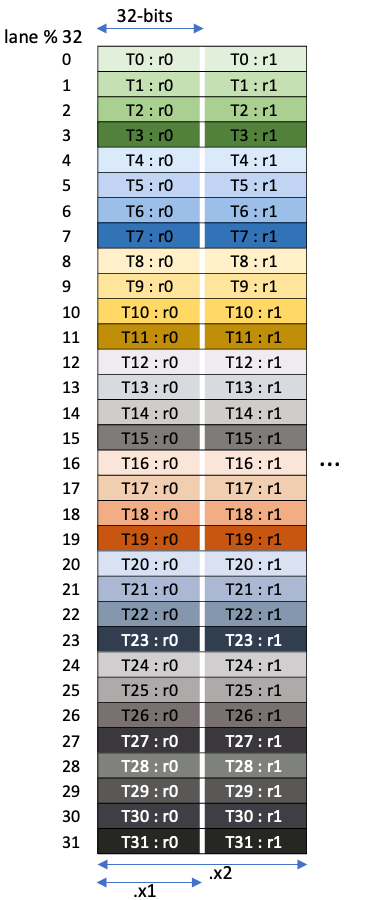
\includegraphics[width=0.3\textwidth]{figures/tikz/wp-tcgen05-tmem-fragment-3232b.png}
    \caption{\texttt{tcgen05\{.ld,.st\}.32x32b.\{x1,x2\}}}
    \label{fig:tmem_fragment-32x32}
\end{subfigure}
\hfill
\begin{subfigure}[b]{0.45\textwidth}
    \centering
    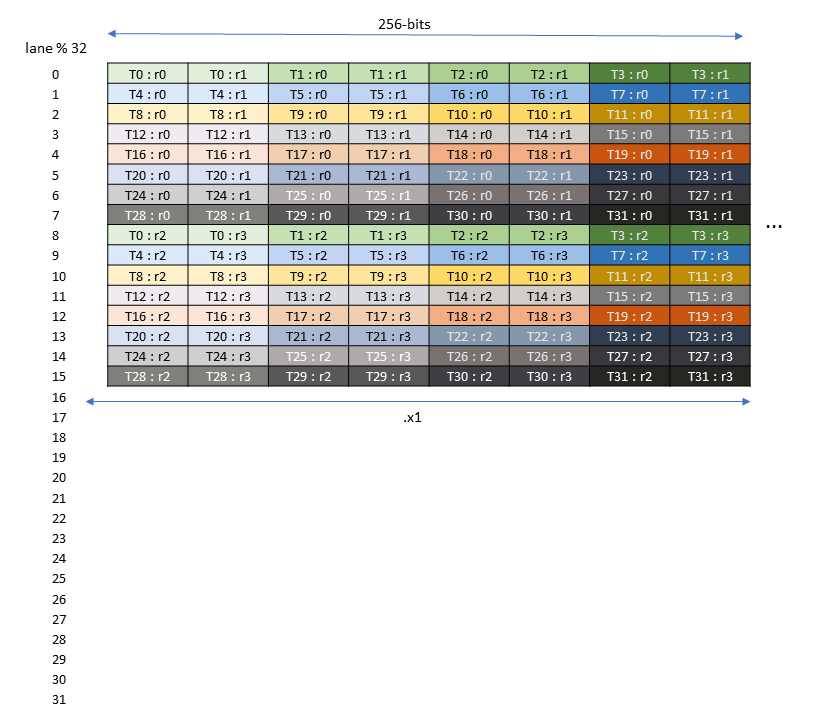
\includegraphics[width=0.8\textwidth]{figures/tikz/wp-tcgen05-tmem-fragment-16256b.png}
    \caption{\texttt{tcgen05\{.ld,.st\}.16x256b.x1}}
    \label{fig:tmem-fragment-16x256}
\end{subfigure}
\caption{TMEM load/store 指令访问特定的偏移，并将数据分配到线程本地寄存器（NVIDIA Corporation 2025）。}
\label{fig:tmem-fragments}
\end{figure}

向 Blackwell 的“张量内存”（tensor memory，TMEM）加载以及从其存储数据所使用的指令，会以一组预定义且非常特定的偏移访问 TMEM，如图~\ref{fig:tmem-fragments} 所示。物理 TMEM 的编址是一个二维网格，最多包含 512 个“列”（col）与 128 个“通道”（lane）。图中是每条指令单个 warp 的访问模式；每条指令实际使用四个 warp，上述模式每 32 个通道重复一次、共重复四次。在对物理 TMEM 编址时，沿 32 位的“列”方向跨越一步使 TMEM 地址增加 1，沿“通道”方向向下跨越一步使 TMEM 地址增加 16384。基于这一物理编址，我们定义记录每条指令所访问的全部物理偏移的布局：
\begin{center}
\begin{tabular}{l | r@{:}l}
\quad\quad\quad\quad \textbf{指令} & \multicolumn{2}{c}{$(\text{指令 COL}, \text{指令 LANE}) \to \text{TMEM 偏移}$} \\
\hline
\texttt{tcgen05\{.ld,.st\}.32x32b.x1} & $(1,128)$ & $(1,16384)$ \\
\texttt{tcgen05\{.ld,.st\}.32x32b.x2} & $(2,128)$ & $(1,16384)$ \\
\texttt{tcgen05\{.ld,.st\}.16x256b.x1} & $(8,(16,4))$ & $(1,(16384,32\cdot 16384))$ \\
\end{tabular}
\end{center}
这些布局与具体指令一一对应，可用来精确确定每条指令将访问 TMEM 中的哪些偏移。

尽管 TMEM 采用二维编址，并被用作形状为 $(M,N)$ 的 MMA 的累加器，TMEM 的“通道”与“列”并不总与逻辑矩阵的行和列相对应。与任何编址方式一样，物理偏移可以通过任意的 \CuTe{} 布局被回绕并折叠成任意形状。因此，给定一个数据布局与一条 TMEM 指令，我们希望确定
\begin{enumerate}[itemsep=0pt,topsep=2pt]
\item 数据布局是否包含该指令将访问的全部偏移；以及
\item 指令所访问的偏移在数据布局中位于何处（以逻辑坐标表示）。
\end{enumerate}

一般地，设数据布局 $\v{A} : \Z(\v{A}) \to \Z_\alpha$ 将逻辑坐标映射到数据偏移，指令布局 $\v{T} : \Z(\v{T}) \to \Z_\beta$ 将指令坐标映射到数据偏移，我们希望确定所有偏移 $\v{T}(i)$ 在 $\v{A}$ 的像中的存在性及其位置。将其表述为
\begin{align*}
\forall i \in \Z_{\abs{\v{T}}}, \exists c \in \Z(\v{A}) \ \ s.t. \ \ \v{T}(i) = \v{A}(c)
\end{align*}
该问题可以通过计算 $\v{A}$ 的左逆并检验下式来高效求解：
\begin{align*}
\v{A}(\v{A}^\dagger(\v{T}(i))) = \v{T}(i)
\end{align*}
也就是说，
\begin{compactitem}
\item 所有偏移 $\v{T}(i)$ 都在 $\v{A}^\dagger$ 的定义域中。
\item 所有坐标 $\v{A}^\dagger(\v{T}(i))$ 都互不相同，且都在 $\v{A}$ 的定义域中。
\end{compactitem}
在这些条件下，我们可以断言：每个偏移 $\v{T}(i)$ 都出现在 $\v{A}$ 的像中，且位于坐标 $\v{A}^\dagger(\v{T}(i))$ 处。布局 $\v{A}^\dagger \circ \v{T}$ 把指令坐标映射到逻辑数据坐标，例如可借助 {\tt zipped\_divide} 把数据布局 $\v{A}$ 切分为与该指令所访问偏移相对应的若干子布局。
